% answers.tex —— 2016 年·全国Ⅱ卷·理科 · 参考答案与详细解析片段
% 由 tools/generate_projects.py 依来源总账自 2016/2016_数学真题_全国2理_试题.md + 2016/2016_数学真题_全国2理_解析正文.md + 2016/2016_数学真题_全国2理_答案要点.md 生成，勿手改（改源 MD 后重跑）


\begin{gktip}
本卷固定原卷不附答案；以下解析根据固定原卷独立整理并经独立复核，非官方解析。第 18(2) 题保留原题语义歧义并关联 ISSUE-0931。
\end{gktip}

\gkpart{选择题}

\begin{answer}
\gksolhead{1}{}

\textbf{题目}：

已知 \(z=(m+3)+(m-1)i\) 在复平面内对应的点在第四象限，则实数 \(m\) 的取值范围是（　）

   (A) \((-3,1)\)　　(B) \((-1,3)\)　　(C) \((1,+\infty)\)　　(D) \((-\infty,-3)\)

\Needspace{4\baselineskip}
\textbf{解析}

复数 \(z=(m+3)+(m-1)i\) 位于第四象限，当且仅当实部为正、虚部为负，即 \(m+3>0\)、\(m-1<0\)。所以 \(-3<m<1\)，选 A。

\gkanswer{答案：A，\((-3,1)\)}

\end{answer}
\begin{answer}
\gksolhead{2}{}

\textbf{题目}：

已知集合 \(A=\{1,2,3\}\)，\(B=\{x\mid(x+1)(x-2)<0,\ x\in\mathbb Z\}\)，则 \(A\cup B=\)（　）

   (A) \(\{1\}\)　　(B) \(\{1,2\}\)　　(C) \(\{0,1,2,3\}\)　　(D) \(\{-1,0,1,2,3\}\)

\Needspace{4\baselineskip}
\textbf{解析}

\((x+1)(x-2)<0\) 的解为 \(-1<x<2\)。其中整数构成 \(B=\{0,1\}\)，故 \(A\cup B=\{1,2,3\}\cup\{0,1\}=\{0,1,2,3\}\)，选 C。

\gkanswer{答案：C，\(\{0,1,2,3\}\)}

\end{answer}
\begin{answer}
\gksolhead{3}{}

\textbf{题目}：

已知向量 \(\boldsymbol a=(1,m),\ \boldsymbol b=(3,-2)\)，且 \((\boldsymbol a+\boldsymbol b)\perp\boldsymbol b\)，则 \(m=\)（　）

   (A) \(-8\)　　(B) \(-6\)　　(C) \(6\)　　(D) \(8\)

\Needspace{4\baselineskip}
\textbf{解析}

\Needspace{5\baselineskip}
\(\boldsymbol a+\boldsymbol b=(4,m-2)\)。由 \((\boldsymbol a+\boldsymbol b)\perp\boldsymbol b\)，得
\nopagebreak[4]
\[
(4,m-2)\cdot(3,-2)=12-2(m-2)=16-2m=0,
\]
所以 \(m=8\)，选 D。

\gkanswer{答案：D，\(m=8\)}

\end{answer}
\begin{answer}
\gksolhead{4}{}

\textbf{题目}：

圆 \(x^2+y^2-2x-8y+13=0\) 的圆心到直线 \(ax+y-1=0\) 的距离为 1，则 \(a=\)（　）

   (A) \(-\dfrac43\)　　(B) \(-\dfrac34\)　　(C) \(\sqrt3\)　　(D) \(2\)

\Needspace{4\baselineskip}
\textbf{解析}

\Needspace{5\baselineskip}
圆方程配方为 \((x-1)^2+(y-4)^2=4\)，圆心为 \((1,4)\)。圆心到直线 \(ax+y-1=0\) 的距离等于 1，故
\nopagebreak[4]
\[
\frac{|a+3|}{\sqrt{a^2+1}}=1.
\]
平方并整理得 \((a+3)^2=a^2+1\)，所以 \(6a+8=0\)，即 \(a=-\frac43\)，选 A。

\gkanswer{答案：A，\(a=-\frac43\)}

\end{answer}
\begin{answer}
\gksolhead{5}{}

\textbf{题目}：

如图，小明从街道的 \(E\) 处出发，先到 \(F\) 处与小红会合，再一起到位于 \(G\) 处的老年公寓参加志愿者活动，则小明到老年公寓可以选择的最短路径条数为（　）
\nopagebreak[4]
\begin{center}% 2016 年全国卷Ⅱ理科第 5 题：街道最短路径图
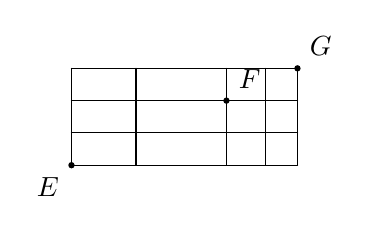
\begin{tikzpicture}[x=0.82cm,y=0.82cm,line cap=round,line join=round]
  % 四列、三行街道网格
  \draw (0,0)--(3.5,0)
        (0,0.5)--(3.5,0.5)
        (0,1.0)--(3.5,1.0)
        (0,1.5)--(3.5,1.5);
  \draw (0,0)--(0,1.5)
        (1.0,0)--(1.0,1.5)
        (2.4,0)--(2.4,1.5)
        (3.0,0)--(3.0,1.5)
        (3.5,0)--(3.5,1.5);
  \fill (0,0) circle (1.15pt);
  \fill (2.4,1.0) circle (1.15pt);
  \fill (3.5,1.5) circle (1.15pt);
  \node[below left=1pt] at (0,0) {$E$};
  \node[above right=1pt] at (2.4,1.0) {$F$};
  \node[above right=1pt] at (3.5,1.5) {$G$};
\end{tikzpicture}
\end{center}
\nopagebreak[4]
   (A) 24　　(B) 18　　(C) 12　　(D) 9

\Needspace{4\baselineskip}
\textbf{解析}

沿街道从 \(E\) 到 \(F\) 需向右 2 格、向上 2 格，最短路线数为 \(\binom42=6\)；从 \(F\) 到 \(G\) 需向右 2 格、向上 1 格，最短路线数为 \(\binom32=3\)。两段可独立衔接，故总数为 \(6\cdot3=18\)，选 B。

\gkanswer{答案：B，18 条}

\end{answer}
\begin{answer}
\gksolhead{6}{}

\textbf{题目}：

如图是由圆柱与圆锥组合而成的几何体的三视图，则该几何体的表面积为（　）
\nopagebreak[4]
\begin{center}% 2016 年全国卷Ⅱ理科第 6 题：圆柱与圆锥组合体的三视图
\begin{tikzpicture}[x=0.55cm,y=0.55cm,>=stealth,line cap=round,line join=round]
  \pgfmathsetmacro{\coneHeight}{2*sqrt(3)}
  % 两个相同的立面轮廓
  \draw (0,0) rectangle (4,4);
  \draw (0,4)--(2,{4+\coneHeight})--(4,4);
  \draw (6,0) rectangle (10,4);
  \draw (6,4)--(8,{4+\coneHeight})--(10,4);

  % 高度尺寸
  \draw[<->] (-0.48,0)--(-0.48,4);
  \draw[<->] (-0.48,4)--(-0.48,{4+\coneHeight});
  \node[left=5pt] at (-0.48,2) {$4$};
  \node[left=5pt] at (-0.48,{4+\coneHeight/2}) {$2\sqrt{3}$};

  % 两个立面底宽尺寸
  \draw (0,0)--(0,-0.48) (4,0)--(4,-0.48);
  \draw[<->] (0,-0.34)--(4,-0.34);
  \node[below=2pt] at (2,-0.34) {$4$};
  \draw (6,0)--(6,-0.48) (10,0)--(10,-0.48);
  \draw[<->] (6,-0.34)--(10,-0.34);
  \node[below=2pt] at (8,-0.34) {$4$};

  % 俯视图及中心点
  \draw (2,-3.3) circle (2);
  \fill (2,-3.3) circle (1.25pt);
\end{tikzpicture}
\end{center}
\nopagebreak[4]
   (A) \(20\pi\)　　(B) \(24\pi\)　　(C) \(28\pi\)　　(D) \(32\pi\)

\Needspace{4\baselineskip}
\textbf{解析}

\Needspace{5\baselineskip}
由三视图得圆柱与圆锥的底面半径均为 2，圆柱高为 4，圆锥高为 \(2\sqrt3\)，圆锥母线长为
\nopagebreak[4]
\[
\sqrt{(2\sqrt3)^2+2^2}=4.
\]
\Needspace{5\baselineskip}
组合体外露面积由圆柱侧面、下底面和圆锥侧面组成：
\nopagebreak[4]
\[
2\pi\cdot2\cdot4+\pi\cdot2^2+\pi\cdot2\cdot4=28\pi,
\]
故选 C。

\gkanswer{答案：C，\(28\pi\)}

\end{answer}
\begin{answer}
\gksolhead{7}{}

\textbf{题目}：

若将函数 \(y=2\sin 2x\) 的图象向左平移 \(\dfrac{\pi}{12}\) 个单位长度，则平移后图象的对称轴为（　）

   (A) \(x=\dfrac{k\pi}{2}-\dfrac{\pi}{6}\ (k\in\mathbb Z)\)　　(B) \(x=\dfrac{k\pi}{2}+\dfrac{\pi}{6}\ (k\in\mathbb Z)\)

   (C) \(x=\dfrac{k\pi}{2}-\dfrac{\pi}{12}\ (k\in\mathbb Z)\)　　(D) \(x=\dfrac{k\pi}{2}+\dfrac{\pi}{12}\ (k\in\mathbb Z)\)

\Needspace{4\baselineskip}
\textbf{解析}

\Needspace{5\baselineskip}
向左平移 \(\frac{\pi}{12}\) 后，函数为 \(y=2\sin(2x+\frac{\pi}{6})\)。对称轴满足 \(2x+\frac{\pi}{6}=\frac{\pi}{2}+k\pi\)，所以
\nopagebreak[4]
\[
x=\frac{k\pi}{2}+\frac{\pi}{6},\qquad k\in\mathbb Z,
\]
选 B。

\gkanswer{答案：B，\(x=\frac{k\pi}{2}+\frac{\pi}{6}\ (k\in\mathbb Z)\)}

\end{answer}
\begin{answer}
\gksolhead{8}{}

\textbf{题目}：

中国古代有计算多项式值的秦九韶算法，如图是实现该算法的程序框图。执行该程序框图，若输入的 \(x=2,n=2\)，依次输入的 \(a\) 为 2，2，5，则输出的 \(s=\)（　）
\nopagebreak[4]
\begin{center}% 2016 年全国卷Ⅱ理科第 8 题：秦九韶算法程序框图
\begin{tikzpicture}[>=stealth,line cap=round,line join=round,font=\small]
  % 开始与输入 x,n
  \draw[rounded corners=4pt] (-0.5,6.94) rectangle (0.5,7.36);
  \node at (0,7.15) {开始};
  \draw (-1.0,6.45)--(-0.8,6.0)--(0.8,6.0)--(1.0,6.45)--cycle;
  \node at (0,6.225) {输入 $x,n$};

  % 初始化、输入 a、循环计算
  \draw (-1.1,4.98) rectangle (1.1,5.48);
  \node at (0,5.23) {$k=0,\ s=0$};
  \draw (-0.82,4.47)--(-0.65,3.97)--(0.65,3.97)--(0.82,4.47)--cycle;
  \node at (0,4.22) {输入 $a$};
  \draw (-1.1,2.55) rectangle (1.1,3.35);
  \node at (0,2.95) {\shortstack{$s=s\cdot x+a$\\$k=k+1$}};

  % 判断、输出与结束
  \draw (0,2.25)--(1.3,1.8)--(0,1.35)--(-1.3,1.8)--cycle;
  \node at (0,1.8) {$k>n$};
  \draw (-0.82,0.8)--(-0.65,0.3)--(0.65,0.3)--(0.82,0.8)--cycle;
  \node at (0,0.55) {输出 $s$};
  \draw[rounded corners=4pt] (-0.5,-0.66) rectangle (0.5,-0.24);
  \node at (0,-0.45) {结束};

  % 主流程与“否”分支回到输入 a
  \draw[->] (0,6.94)--(0,6.45);
  \draw[->] (0,6.0)--(0,5.48);
  \draw (0,4.98)--(0,4.72);
  \draw[->] (0,4.72)--(0,4.47);
  \draw[->] (0,3.97)--(0,3.35);
  \draw[->] (0,2.55)--(0,2.2);
  \draw[->] (0,1.4)--(0,0.8);
  \draw[->] (0,0.3)--(0,-0.24);
  \draw (1.3,1.8)--(2.25,1.8)--(2.25,4.72)--(0,4.72);
  \node[right=2pt] at (1.3,2.0) {否};
  \node[right=3pt] at (0,1.08) {是};
\end{tikzpicture}
\end{center}
\nopagebreak[4]
   (A) 7　　(B) 12　　(C) 17　　(D) 34

\Needspace{4\baselineskip}
\textbf{解析}

流程图从 \(s=0,k=0\) 开始，每轮先令 \(s\leftarrow sx+a\)，再令 \(k\leftarrow k+1\)，当 \(k>n=2\) 时停止。输入 \(a=2,2,5\) 后，\(s\) 依次为 \(2,6,17\)，故输出 17，选 C。

\gkanswer{答案：C，17}

\end{answer}
\begin{answer}
\gksolhead{9}{}

\textbf{题目}：

若 \(\cos\left(\dfrac\pi4-\alpha\right)=\dfrac35\)，则 \(\sin 2\alpha=\)（　）

   (A) \(\dfrac7{25}\)　　(B) \(\dfrac15\)　　(C) \(-\dfrac15\)　　(D) \(-\dfrac7{25}\)

\Needspace{4\baselineskip}
\textbf{解析}

\Needspace{5\baselineskip}
令 \(\theta=\frac{\pi}{4}-\alpha\)，则 \(\cos\theta=\frac35\)。于是
\nopagebreak[4]
\[
\sin2\alpha=\sin\left(\frac\pi2-2\theta\right)=\cos2\theta
=2\cos^2\theta-1=-\frac7{25},
\]
选 D。

\gkanswer{答案：D，\(-\frac7{25}\)}

\end{answer}
\begin{answer}
\gksolhead{10}{}

\textbf{题目}：

从区间 \([0,1]\) 随机抽取 \(2n\) 个数 \(x_1,\allowbreak x_2,\allowbreak\cdots,\allowbreak x_n,\allowbreak y_1,\allowbreak y_2,\allowbreak\cdots,\allowbreak y_n\)，构成 \(n\) 个数对 \((x_1,y_1),\allowbreak(x_2,y_2),\allowbreak\cdots,\allowbreak(x_n,y_n)\)，其中两数的平方和小于 1 的数对共有 \(m\) 个，则用随机模拟的方法得到的圆周率的近似值为（　）

   (A) \(\dfrac{4n}{m}\)　　(B) \(\dfrac{2n}{m}\)　　(C) \(\dfrac{4m}{n}\)　　(D) \(\dfrac{2m}{n}\)

\Needspace{4\baselineskip}
\textbf{解析}

每个随机数对均匀分布在单位正方形 \([0,1]^2\) 内。满足 \(x^2+y^2<1\) 的点构成四分之一单位圆，概率为 \(\pi/4\)。模拟频率近似为 \(m/n\)，因此 \(\pi\approx4m/n\)，选 C。

\gkanswer{答案：C，\(\frac{4m}{n}\)}

\end{answer}
\begin{answer}
\gksolhead{11}{}

\textbf{题目}：

已知 \(F_1,F_2\) 是双曲线 \(E:\dfrac{x^2}{a^2}-\dfrac{y^2}{b^2}=1\) 的左、右焦点，点 \(M\) 在 \(E\) 上，\(MF_1\) 与 \(x\) 轴垂直，\(\sin\angle MF_2F_1=\dfrac13\)，则 \(E\) 的离心率为（　）

   (A) \(\sqrt2\)　　(B) \(\dfrac32\)　　(C) \(\sqrt3\)　　(D) \(2\)

\Needspace{4\baselineskip}
\textbf{解析}

\Needspace{5\baselineskip}
设双曲线焦距参数为 \(c\)，离心率为 \(e=c/a>1\)。因 \(MF_1\perp x\) 轴，\(M\) 与左焦点 \(F_1=(-c,0)\) 有相同横坐标；代入双曲线得 \(|MF_1|=b^2/a=a(e^2-1)\)。又 \(F_1F_2=2c=2ae\)，故直角三角形 \(MF_1F_2\) 中
\nopagebreak[4]
\[
\sin\angle MF_2F_1=\frac{e^2-1}{e^2+1}=\frac13.
\]
解得 \(e^2=2\)，所以离心率 \(e=\sqrt2\)，选 A。

\gkanswer{答案：A，\(\sqrt2\)}

\end{answer}
\begin{answer}
\gksolhead{12}{}

\textbf{题目}：

已知函数 \(f(x)\ (x\in\mathbb R)\) 满足 \(f(-x)=2-f(x)\)，若函数 \(y=\dfrac{x+1}{x}\) 与 \(y=f(x)\) 图象的交点为 \((x_1,y_1),(x_2,y_2),\cdots,(x_m,y_m)\)，则 \(\displaystyle\sum_{i=1}^m(x_i+y_i)=\)（　）

   (A) 0　　(B) \(m\)　　(C) \(2m\)　　(D) \(4m\)

\Needspace{4\baselineskip}
\textbf{解析}

若 \((x,y)\) 是两图象的交点，由 \(f(-x)=2-f(x)\) 可知 \((-x,2-y)\) 也在 \(y=f(x)\) 上。又当 \(y=1+\frac1x\) 时，\(2-y=1-\frac1x=\frac{-x+1}{-x}\)，所以该点也在 \(y=1+\frac1x\) 上。交点成对出现，每对的两个 \(x\) 坐标和为 0、两个 \(y\) 坐标和为 2，总和等于交点个数 \(m\)，选 B。

\gkanswer{答案：B，\(m\)}

\end{answer}
\gkpart{填空题}

\begin{answer}
\gksolhead{13}{}

\textbf{题目}：

\(\triangle ABC\) 的内角 \(A,B,C\) 的对边分别为 \(a,b,c\)，若 \(\cos A=\dfrac45,\ \cos C=\dfrac5{13},\ a=1\)，则 \(b=\underline{\qquad\qquad}\)。

\Needspace{4\baselineskip}
\textbf{解析}

\Needspace{5\baselineskip}
由 \(\cos A=\frac45\)、\(\cos C=\frac5{13}\)，且 \(A,C\) 为三角形内角，得 \(\sin A=\frac35\)、\(\sin C=\frac{12}{13}\)。又 \(B=\pi-(A+C)\)，从而
\nopagebreak[4]
\[
\sin B=\sin(A+C)=\frac35\cdot\frac5{13}+\frac45\cdot\frac{12}{13}=\frac{63}{65}.
\]
由正弦定理及 \(a=1\)，得 \(b=a\frac{\sin B}{\sin A}=\frac{21}{13}\)。

\gkanswer{答案：\(\frac{21}{13}\)}

\end{answer}
\begin{answer}
\gksolhead{14}{}

\textbf{题目}：

\(\alpha,\beta\) 是两个平面，\(m,n\) 是两条线，有下列四个命题：

   ① 如果 \(m\perp n,\ m\perp\alpha,\ n\parallel\beta\)，那么 \(\alpha\perp\beta\)；

   ② 如果 \(m\perp\alpha,\ n\parallel\alpha\)，那么 \(m\perp n\)；

   ③ 如果 \(\alpha\parallel\beta,\ m\subset\alpha\)，那么 \(m\parallel\beta\)；

   ④ 如果 \(m\parallel n,\ \alpha\parallel\beta\)，那么 \(m\) 与 \(\alpha\) 所成的角和 \(n\) 与 \(\beta\) 所成的角相等。

   则上述四个命题中真命题的是\(\underline{\qquad\qquad}\)。

\Needspace{4\baselineskip}
\textbf{解析}

命题①不成立：取 \(\alpha=\beta\) 为水平面，令 \(m\) 为其法线、\(n\) 为与平面平行且不在平面内的水平直线，则前件成立而 \(\alpha\not\perp\beta\)。②由线面垂直的性质成立；③因 \(\alpha\parallel\beta\) 且 \(m\subset\alpha\)，有 \(m\parallel\beta\)；④平行直线与平行平面所成角相等。因此真命题为②③④。

\gkanswer{答案：②③④}

\end{answer}
\begin{answer}
\gksolhead{15}{}

\textbf{题目}：

有三张卡片，分别写有 1 和 2，1 和 3，2 和 3。甲、乙、丙三人各取走一张卡片，甲看了乙的卡片后说：“我与乙的卡片上相同的数字不是 2”，乙看了丙的卡片后说：“我与丙的卡片上相同的数字不是 1”，丙说：“我的卡片上的数字之和不是 5”，则甲的卡片上的数字是\(\underline{\qquad\qquad}\)。

\Needspace{4\baselineskip}
\textbf{解析}

丙的卡片数字和不为 5，所以丙不拿 \(\{2,3\}\)。若丙拿 \(\{1,3\}\)，乙为满足“与丙共有的数字不是 1”只能拿 \(\{2,3\}\)，剩下甲拿 \(\{1,2\}\)，这会使甲乙共有 2，与甲的陈述矛盾。因此丙拿 \(\{1,2\}\)，乙拿 \(\{2,3\}\)，甲拿 \(\{1,3\}\)。

\gkanswer{答案：甲拿 \(\{1,3\}\)}

\end{answer}
\begin{answer}
\gksolhead{16}{}

\textbf{题目}：

若直线 \(y=kx+b\) 是曲线 \(y=\ln x+2\) 的切线，也是曲线 \(y=\ln(x+1)\) 的切线，\(b=\underline{\qquad\qquad}\)。

\Needspace{4\baselineskip}
\textbf{解析}

\Needspace{5\baselineskip}
设两曲线切点横坐标分别为 \(u>0\)、\(v>-1\)。第一条曲线的切线斜率和截距为 \(1/u\)、\(\ln u+1\)；第二条曲线的切线斜率和截距为 \(1/(v+1)\)、\(\ln(v+1)-v/(v+1)\)。两切线重合要求 \(u=v+1\)。令共同斜率为 \(k=1/u\)，截距相等化为
\nopagebreak[4]
\[
1-\ln k=-\ln k-1+k,
\]
故 \(k=2\)、\(u=\frac12\)，直线截距 \(b=\ln(\frac12)+1=1-\ln2\)。

\gkanswer{答案：\(b=1-\ln2\)}

\end{answer}
\gkpart{解答题}

\begin{answer}
\gksolhead{17}{}

\textbf{题目}：

\(S_n\) 为等差数列 \(\{a_n\}\) 的前 \(n\) 项和，且 \(a_1=1,\ S_7=28\)。记 \(b_n=\lfloor\lg a_n\rfloor\)，其中 \(\lfloor x\rfloor\) 表示不超过 \(x\) 的最大整数，如 \(\lfloor0.9\rfloor=0,\ \lfloor\lg99\rfloor=1\)。

   (1) 求 \(b_1,b_{11},b_{101}\)；

   (2) 求数列 \(\{b_n\}\) 的前 1000 项和。

\Needspace{4\baselineskip}
\textbf{解析}

\gksubpart{(1)}

由 \(S_7=7a_1+21d=28\) 且 \(a_1=1\)，得公差 \(d=1\)，所以 \(a_n=n\)、\(b_n=\lfloor\lg n\rfloor\)。因此 \(b_1=0\)、\(b_{11}=1\)、\(b_{101}=2\)。

\gksubpart{(2)}

\Needspace{5\baselineskip}
在 \(1\le n\le9\) 时 \(\lfloor\lg n\rfloor=0\)；\(10\le n\le99\) 共 90 项取 1；\(100\le n\le999\) 共 900 项取 2；\(n=1000\) 时取 3。因此
\nopagebreak[4]
\[
\sum_{n=1}^{1000}b_n=90+2\cdot900+3=1893.
\]

\gkanswer{答案（1）：\(b_1=0,\ b_{11}=1,\ b_{101}=2\)}

\gkanswer{答案（2）：\(1893\)}

\end{answer}
\begin{answer}
\gksolhead{18}{}

\textbf{题目}：

某险种的基本保费为 \(a\)（单位：元），继续购买该险种的投保人称为续保人，续保人本年度的保费与其上年度出险次数的关联如下：

\begin{center}
\begin{tabular}{lrrrrrr}
\toprule
上年度出险次数 & 0 & 1 & 2 & 3 & 4 & \(\geq5\) \\
\midrule
保费 & \(0.85a\) & \(a\) & \(1.25a\) & \(1.5a\) & \(1.75a\) & \(2a\) \\
\bottomrule
\end{tabular}
\end{center}

设该险种一续保人一年内出险次数与相应概率如下：

\begin{center}
\begin{tabular}{lrrrrrr}
\toprule
一年内出险次数 & 0 & 1 & 2 & 3 & 4 & \(\geq5\) \\
\midrule
概率 & 0.30 & 0.15 & 0.20 & 0.20 & 0.10 & 0.05 \\
\bottomrule
\end{tabular}
\end{center}

   (1) 求一续保人本年度的保费高于基本保费的概率；

   (2) 若一续保人本年度的保费高于基本保费，求其保费比基本保费高出 60\% 的概率；

   (3) 求续保人本年度的平均保费与基本保费的比值。

\Needspace{4\baselineskip}
\textbf{解析}

\gksubpart{(1)}

\Needspace{5\baselineskip}
记上年度出险次数为 \(X\)。本年度保费高于基本保费 \(a\) 当且仅当 \(X\ge2\)，故
\nopagebreak[4]
\[
P(X\ge2)=0.20+0.20+0.10+0.05=0.55.
\]

\gksubpart{(2)}

\Needspace{5\baselineskip}
已知本年度保费高于 \(a\)，即 \(X\ge2\)。若“高出基本保费 60\%”按恰好增加基本保费的 \(0.6a\) 理解，需要保费为 \(1.6a\)，但表中不存在这一档，条件概率为 0。若按至少增加基本保费的 \(0.6a\) 理解，则保费为 \(1.75a\) 或 \(2a\)，对应 \(X\ge4\)，条件概率为
\nopagebreak[4]
\[
P(X\ge4\mid X\ge2)=\frac{0.10+0.05}{0.20+0.20+0.10+0.05}=\frac3{11}.
\]
原题未说明采用等值事件还是阈值事件，且现有考试评析未给出事件定义，故不把任一结果作为唯一答案；本小问标 U，关联 ISSUE-0931。

\gksubpart{(3)}

\Needspace{5\baselineskip}
以基本保费 \(a\) 为单位，年平均保费与基本保费之比为
\nopagebreak[4]
\[
0.30(0.85)+0.15(1)+0.20(1.25)+0.20(1.5)+0.10(1.75)+0.05(2)=1.23=\frac{123}{100}.
\]

\gkanswer{答案（1）：\(0.55\)}

\gkanswer{答案（2）：U}

\gkanswer{答案（3）：\(\frac{123}{100}=1.23\)}

\end{answer}
\begin{answer}
\gksolhead{19}{}

\textbf{题目}：

如图，菱形 \(ABCD\) 的对角线 \(AC\) 与 \(BD\) 交于点 \(O\)，\(AB=5,\ AC=6\)，点 \(E,F\) 分别在 \(AD,CD\) 上，\(AE=CF=\dfrac54\)，\(EF\) 交 \(BD\) 于点 \(H\)。将三角形 \(DEF\) 沿 \(EF\) 折到三角形 \(D'EF\) 的位置，\(OD'=\sqrt{10}\)。
\nopagebreak[4]
\begin{center}% 2016 年全国卷Ⅱ理科第 19 题：菱形底面与折起后的 D'
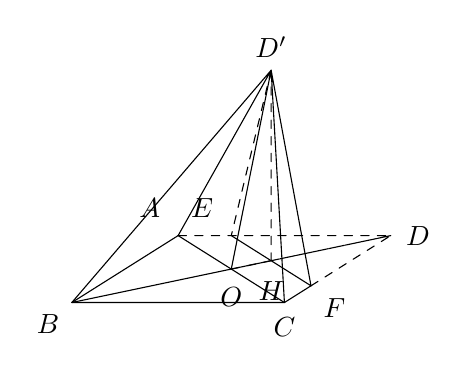
\begin{tikzpicture}[line cap=round,line join=round]
  \coordinate (A)  at (0,1.1);
  \coordinate (B)  at (-1.35,0.25);
  \coordinate (C)  at (1.35,0.25);
  \coordinate (D)  at (2.7,1.1);
  \coordinate (O)  at (0.675,0.675);
  \coordinate (E)  at (0.675,1.1);
  \coordinate (F)  at (1.6875,0.4625);
  \coordinate (H)  at (1.18125,0.78125);
  \coordinate (Dp) at (1.18125,3.2);

  % 按原图保留虚线段，不另作线型含义解释
  \draw[dashed] (A)--(D) (F)--(D) (H)--(D) (Dp)--(H) (Dp)--(E) (O)--(D);

  % 菱形、对角线、折痕与折起后的连线
  \draw (A)--(B)--(C);
  \draw (A)--(C);
  \draw (B)--(H);
  \draw (E)--(F);
  \draw (C)--(F);
  \draw (Dp)--(A) (Dp)--(B) (Dp)--(C) (Dp)--(F) (Dp)--(O);

  \node[above left=3pt] at (A) {$A$};
  \node[below left=1pt] at (B) {$B$};
  \node[below=2pt] at (C) {$C$};
  \node[right=2pt] at (D) {$D$};
  \node[above left=3pt] at (E) {$E$};
  \node[below right=1pt] at (F) {$F$};
  \node[below=3pt] at (O) {$O$};
  \node[below=4pt] at (H) {$H$};
  \node[above=1pt] at (Dp) {$D'$};
\end{tikzpicture}
\end{center}
\nopagebreak[4]
   (1) 证明：\(D'H\perp\) 平面 \(ABCD\)；

   (2) 求二面角 \(B-D'-A-C\) 的正弦值。

\Needspace{4\baselineskip}
\textbf{解析}

\gksubpart{(1)}

\Needspace{5\baselineskip}
取底面位于 \(z=0\)，设
\nopagebreak[4]
\[
O=(0,0,0),\quad A=(-3,0,0),\quad C=(3,0,0),\quad B=(0,4,0),\quad D=(0,-4,0).
\]
由 \(AE=CF=\frac54\)，得 \(E=(-\frac94,-1,0)\)、\(F=(\frac94,-1,0)\)，所以 \(EF\) 的中点 \(H=(0,-1,0)\)，且 \(DH=3\)、\(OH=1\)。折叠后 \(E,F\) 不动；由于 \(DE=DF\)，点 \(D'\) 在 \(EF\) 的垂直平分面内。该平面由 \(BD\) 与垂直于底面的方向张成。折叠保持长度，故 \(D'H=DH=3\)；又 \(OD'=\sqrt{10}\)，于是 \(OD'^2=OH^2+D'H^2\)，三角形 \(OHD'\) 在 \(H\) 处直角，故 \(D'H\perp BD\)。在上述垂直平分面内，垂直于 \(BD\) 的方向垂直于底面，因此 \(D'H\perp\) 平面 \(ABCD\)。

\gksubpart{(2)}

\Needspace{5\baselineskip}
可取折后 \(D'=(0,-1,3)\)。平面 \(BD'A\)、\(D'AC\) 的法向量可分别取
\nopagebreak[4]
\[
\boldsymbol n_1=(-4,3,5),\qquad \boldsymbol n_2=(0,3,1).
\]
\Needspace{5\baselineskip}
其模分别为 \(\sqrt{50}\)、\(\sqrt{10}\)，内积绝对值为 14。故两平面夹角的余弦绝对值为
\nopagebreak[4]
\[
\frac{|\boldsymbol n_1\cdot\boldsymbol n_2|}{\|\boldsymbol n_1\|\|\boldsymbol n_2\|}=\frac{14}{\sqrt{50}\sqrt{10}}=\frac7{5\sqrt5}.
\]
\Needspace{5\baselineskip}
所求正弦为
\nopagebreak[4]
\[
\sqrt{1-\frac{49}{125}}=\frac{2\sqrt{95}}{25}.
\]

\gkanswer{答案（1）：\(D'H\perp\) 平面 \(ABCD\)}

\gkanswer{答案（2）：\(\sin\) 二面角 \(B-D'-A-C=\frac{2\sqrt{95}}{25}\)}

\end{answer}
\begin{answer}
\gksolhead{20}{}

\textbf{题目}：

已知椭圆 \(E:\dfrac{x^2}{t}+\dfrac{y^2}{3}=1\) 的焦点在 \(x\) 轴上，\(A\) 是 \(E\) 的左顶点，斜率为 \(k\ (k>0)\) 的直线交 \(E\) 于 \(A,M\) 两点，点 \(N\) 在 \(E\) 上，\(MA\perp NA\)。

   (1) 当 \(t=4,\ |AM|=|AN|\) 时，求三角形 \(AMN\) 的面积；

   (2) 当 \(2|AM|=|AN|\) 时，求 \(k\) 的取值范围。

\Needspace{4\baselineskip}
\textbf{解析}

\gksubpart{(1)}

\Needspace{5\baselineskip}
记 \(p=\sqrt t>\sqrt3\)，则左顶点 \(A=(-p,0)\)。从 \(A\) 出发斜率为 \(s\) 的弦，其另一端相对 \(A\) 的位移可写成 \((v,sv)\)。代入椭圆 \(x^2/t+y^2/3=1\)，得
\nopagebreak[4]
\[
v=\frac{6p}{3+p^2s^2},\qquad |A P_s|=\frac{6p\sqrt{1+s^2}}{3+p^2s^2}.
\]
\Needspace{5\baselineskip}
两条互相垂直的弦斜率为 \(k\) 与 \(-1/k\)，所以
\nopagebreak[4]
\[
\frac{|AN|}{|AM|}=\frac{k(3+p^2k^2)}{3k^2+p^2}.
\]
\Needspace{5\baselineskip}
当 \(t=p^2=4\) 且两弦等长时，\((k-1)(4k^2+k+4)=0\)。因 \(k>0\)，得 \(k=1\)。此时 \(|AM|=\frac{12\sqrt2}{7}\)，三角形 \(AMN\) 为直角等腰三角形，面积为
\nopagebreak[4]
\[
\frac12|AM|^2=\frac{144}{49}.
\]

\gksubpart{(2)}

\Needspace{5\baselineskip}
条件 \(|AN|=2|AM|\) 化为
\nopagebreak[4]
\[
t(k^3-2)=3k(2k-1),\qquad t=\frac{3k(2k-1)}{k^3-2}.
\]
\Needspace{5\baselineskip}
要求 \(t>3\)。若 \(0<k<\sqrt[3]2\)，为使 \(t>0\) 必须 \(0<k<\frac12\)，但此时 \(t<3\)，不合条件。若 \(k>\sqrt[3]2\)，则
\nopagebreak[4]
\[
t-3=-\frac{3(k-2)(k^2+1)}{k^3-2}>0
\]
当且仅当 \(k<2\)。因此取值范围为 \(\sqrt[3]2<k<2\)。

\gkanswer{答案（1）：\(\frac{144}{49}\)}

\gkanswer{答案（2）：\(\sqrt[3]{2}<k<2\)}

\end{answer}
\begin{answer}
\gksolhead{21}{}

\textbf{题目}：

(1) 讨论函数 \(f(x)=\dfrac{x-2}{x+2}\cdot e^x\) 的单调性，并证明当 \(x>0\) 时，\((x-2)e^x+x+2>0\)；

   (2) 证明：当 \(a\in[0,1)\) 时，函数 \(g(x)=\dfrac{e^x-ax-a}{x^2}\ (x>0)\) 有最小值。设 \(g(x)\) 的最小值为 \(h(a)\)，求函数 \(h(a)\) 的值域。

\Needspace{4\baselineskip}
\textbf{解析}

\gksubpart{(1)}

\Needspace{5\baselineskip}
在定义域 \(x\ne-2\) 上，
\nopagebreak[4]
\[
f'(x)=\frac{x^2e^x}{(x+2)^2}\ge0.
\]
导数除 \(x=0\) 外为正，因此 \(f\) 在 \((-\infty,-2)\) 与 \((-2,+\infty)\) 上分别严格递增。令 \(q(x)=(x-2)e^x+x+2\)，则 \(q(0)=q'(0)=0\)，且 \(q''(x)=xe^x>0\)（\(x>0\)）。故先有 \(q'(x)>0\)，继而 \(q(x)>0\)，即题设不等式成立。

\gksubpart{(2)}

\Needspace{5\baselineskip}
令
\nopagebreak[4]
\[
N_a(x)=(x-2)e^x+a(x+2),\qquad g'(x)=\frac{N_a(x)}{x^3}.
\]
对 \(0\le a<1\)，有 \(N_a(0)=2(a-1)<0\)、\(N_a'(0)=a-1<0\)，而 \(N_a'(x)\to+\infty\)。又 \(N_a''(x)=xe^x>0\)（\(x>0\)），所以 \(N_a'\) 严格递增并恰有一个零点；相应地 \(N_a\) 先减后增。结合 \(N_a(0)<0\)、\(N_a(x)\to+\infty\)，\(N_a\) 恰有一个正零点 \(x_a\)。于是 \(g\) 先减后增。再由 \(g(x)\to+\infty\)（\(x\to0^+\) 或 \(x\to+\infty\)），最小值存在。

\Needspace{5\baselineskip}
驻点方程给出
\nopagebreak[4]
\[
a=\frac{(2-x_a)e^{x_a}}{x_a+2},\qquad h(a)=g(x_a)=\frac{e^{x_a}}{x_a+2}.
\]
\Needspace{5\baselineskip}
右侧第一式关于 \(x_a\in(0,2]\) 严格递减，故当 \(a\) 从 0 增至但不达 1 时，\(x_a\) 从 2 降至但不达 0。函数 \(e^x/(x+2)\) 在 \(x>0\) 上严格递增，因而
\nopagebreak[4]
\[
h(a)\in\left(\frac12,\frac{e^2}{4}\right].
\]

\gkanswer{答案（1）：\(f\) 在 \((-\infty,-2)\)、\((-2,+\infty)\) 上分别严格递增；当 \(x>0\) 时，\((x-2)e^x+x+2>0\)。}

\gkanswer{答案（2）：\(\left(\frac12,\frac{e^2}{4}\right]\)}

\end{answer}
\begin{answer}
\gksolhead{22}{}

\textbf{题目}：

如图，在正方形 \(ABCD\) 中，\(E,G\) 分别在边 \(DA,DC\) 上（不与端点重合），且 \(DE=DG\)，过 \(D\) 点作 \(DF\perp CE\)，垂足为 \(F\)。
\nopagebreak[4]
\begin{center}% 2016 年全国卷Ⅱ理科第 22 题：正方形内的垂足与连线
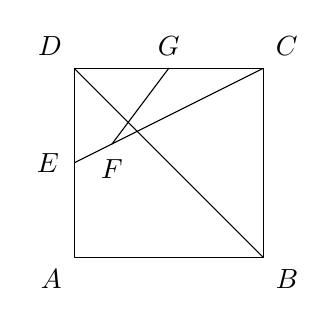
\begin{tikzpicture}[line cap=round,line join=round]
  \coordinate (A) at (0,0);
  \coordinate (B) at (2.4,0);
  \coordinate (C) at (2.4,2.4);
  \coordinate (D) at (0,2.4);
  \coordinate (E) at (0,1.2);
  \coordinate (G) at (1.2,2.4);
  \coordinate (F) at (0.48,1.44);

  \draw (A)--(B)--(C)--(D)--cycle;
  \draw (D)--(B);
  \draw (E)--(C);
  \draw (F)--(G);

  \node[below left=1pt] at (A) {$A$};
  \node[below right=1pt] at (B) {$B$};
  \node[above right=1pt] at (C) {$C$};
  \node[above left=1pt] at (D) {$D$};
  \node[left=2pt] at (E) {$E$};
  \node[above=1pt] at (G) {$G$};
  \node[below=2pt] at (F) {$F$};
\end{tikzpicture}
\end{center}
\nopagebreak[4]
   (1) 证明：\(B,C,G,F\) 四点共圆；

   (2) 若 \(AB=1,\ E\) 为 \(DA\) 的中点，求四边形 \(BCGF\) 的面积。

\Needspace{4\baselineskip}
\textbf{解析}

\gksubpart{(1)}

\Needspace{5\baselineskip}
令 \(D=(0,0)\)、\(C=(1,0)\)、\(A=(0,-1)\)、\(B=(1,-1)\)，设 \(DE=DG=s\in(0,1)\)，则 \(E=(0,-s)\)、\(G=(s,0)\)。直线 \(CE\) 的方向向量为 \((1,s)\)，从 \(D\) 向其作垂线的垂足为
\nopagebreak[4]
\[
F=\left(\frac{s^2}{1+s^2},-\frac{s}{1+s^2}\right).
\]
\Needspace{5\baselineskip}
过 \(B,C,G\) 的圆方程为
\nopagebreak[4]
\[
x^2+y^2-(s+1)x+y+s=0.
\]
将 \(F\) 的坐标代入亦满足该方程，故 \(B,C,G,F\) 四点共圆。

\gksubpart{(2)}

当 \(AB=1\)、\(E\) 为 \(DA\) 中点时 \(s=\frac12\)，所以 \(G=(\frac12,0)\)、\(F=(\frac15,-\frac25)\)。按顶点顺序 \(B,C,G,F\) 用鞋带公式，得到四边形 \(BCGF\) 面积为 \(\frac12\)。

\gkanswer{答案（1）：\(B,C,G,F\) 四点共圆}

\gkanswer{答案（2）：\(\frac12\)}

\end{answer}
\begin{answer}
\gksolhead{23}{}

\textbf{题目}：

在直角坐标系 \(xOy\) 中，圆 \(C\) 的方程为 \((x+6)^2+y^2=25\)。

   (1) 以坐标原点为极点，\(x\) 轴正半轴为极轴建立极坐标系，求圆 \(C\) 的极坐标方程；

   (2) 直线 \(l\) 的参数方程是 \(\begin{cases}x=t\cos\alpha,\\y=t\sin\alpha,\end{cases}\)（\(t\) 为参数），直线 \(l\) 与圆 \(C\) 交于 \(A,B\) 两点，\(|AB|=\sqrt{10}\)，求 \(l\) 的斜率。

\Needspace{4\baselineskip}
\textbf{解析}

\gksubpart{(1)}

\Needspace{5\baselineskip}
代入 \(x=\rho\cos\theta\)、\(y=\rho\sin\theta\) 到 \((x+6)^2+y^2=25\)，得
\nopagebreak[4]
\[
\rho^2+12\rho\cos\theta+36=25,
\]
所以极坐标方程为 \(\rho^2+12\rho\cos\theta+11=0\)。

\gksubpart{(2)}

\Needspace{5\baselineskip}
令过原点直线的单位方向向量为 \((\cos\alpha,\sin\alpha)\)，交点参数 \(t\) 满足
\nopagebreak[4]
\[
t^2+12t\cos\alpha+11=0.
\]
\Needspace{5\baselineskip}
两交点在该直线上的距离为两根之差的绝对值，即判别式的平方根。因此
\nopagebreak[4]
\[
|AB|^2=144\cos^2\alpha-44=10,
\]
\Needspace{5\baselineskip}
从而 \(\cos^2\alpha=\frac38\)、\(\sin^2\alpha=\frac58\)，故直线斜率满足
\nopagebreak[4]
\[
\tan\alpha=\pm\sqrt{\frac53}=\pm\frac{\sqrt{15}}3.
\]
题面允许两种斜率，完整答案为这两个值。

\gkanswer{答案（1）：\(\rho^2+12\rho\cos\theta+11=0\)}

\gkanswer{答案（2）：斜率为 \(\pm\frac{\sqrt{15}}3\)}

\end{answer}
\begin{answer}
\gksolhead{24}{}

\textbf{题目}：

已知函数 \(f(x)=\left|x-\dfrac12\right|+\left|x+\dfrac12\right|\)，\(M\) 为不等式 \(f(x)<2\) 的解集。

   (1) 求 \(M\)；

   (2) 证明：当 \(a,b\in M\) 时，\(|a+b|<|1+ab|\)。

\Needspace{4\baselineskip}
\textbf{解析}

\gksubpart{(1)}

\Needspace{5\baselineskip}
由绝对值分段可得
\nopagebreak[4]
\[
f(x)=\begin{cases}
-2x,&x\le-\frac12,\\
1,&-\frac12\le x\le\frac12,\\
2x,&x\ge\frac12.
\end{cases}
\]
所以 \(f(x)<2\) 等价于 \(-1<x<1\)，即 \(M=(-1,1)\)。

\gksubpart{(2)}

\Needspace{5\baselineskip}
若 \(a,b\in(-1,1)\)，则
\nopagebreak[4]
\[
(1+ab)+(a+b)=(1+a)(1+b)>0,
\]
\nopagebreak[4]
\[
(1+ab)-(a+b)=(1-a)(1-b)>0.
\]
因此 \(1+ab>|a+b|\)，且 \(1+ab>0\)，故 \(|a+b|<|1+ab|\)。

\gkanswer{答案（1）：\(M=(-1,1)\)}

\gkanswer{答案（2）：\(|a+b|<|1+ab|\)}

\end{answer}